\documentclass[UTF-8,a4paper,zihao=-4]{ctexart}
\usepackage[a4paper,left=3cm,right=2.5cm,top=3cm,bottom=2.5cm]{geometry}
\usepackage{graphicx} % Required for inserting images
\usepackage[backend=biber,style=gb7714-2015]{biblatex} 
\addbibresource{ref.bib} %待补上参考文献 
\usepackage{amsmath,amssymb}   % 公式
\usepackage{graphicx}          % 插图
\usepackage{booktabs}           % 三线表
\usepackage{hyperref}           % 超链接（最后加载，少数例外）
\usepackage{placeins}
\pagestyle{plain} 
\ctexset{
  section = {
    number = \chinese{section},   % 中文数字：一、二、三…
    format = \zihao{3}\heiti\centering,
    aftername = \quad,            % 编号和标题之间的空格（可调）
    % 如果你想变成“一、绪论”（带顿号），把 aftername 改成 \hspace{1em} 或直接写顿号
  }
}
\makeatletter
\renewcommand{\maketitle}{
    \begin{center}
        \vspace*{-2cm}
        {\zihao{2}\heiti\@title\par}
    \end{center}
}
\makeatother

\makeatletter
\renewenvironment{abstract}
{
    \begin{center}
        {\zihao{-3}\textbf{摘要}}
    \end{center}
    \zihao{-4}
}
{}
\makeatother

\begin{document}

\title{“板凳龙”闹元宵}
\date{}
\maketitle


%%%%%摘要%%%%%
\begin{abstract}

“板凳龙”，又称“盘龙”，是浙闽地区的传统地方民俗文化活动，人们将数十条板凳相连，以圆盘状进行“盘龙”活动。因此，本文集中研究“盘龙”活动中的“盘入”与“盘出”行为，并研究龙头与龙身之间的关系。
    
\textbf{针对问题一：} 本文将舞龙队盘入过程抽象为\textbf{等距螺线参数化运动模型，建立极坐标系}，利用螺线弧长与参数角的关系，将龙头匀速运动转化为\textbf{弧长—角度数值反解问题}，确定龙头位置随时间的变化。在此基础上，根据板凳间固定连接约束，建立\textbf{前向递推模型}，逐节求解各把手位置，并通过参数变化关系建立\textbf{速度递推模型}，最终实现舞龙队在给定时间范围内的位置与速度求解。
    
\textbf{针对问题二：} 本文在问题一运动模型基础上，引入板凳尺寸约束，建立\textbf{矩形刚体碰撞模型}。根据舞龙盘入特点，以龙头板凳为主要检测对象，通过螺线参数关系筛选\textbf{候选碰撞板凳集合}，并采用\textbf{分离轴定理（SAT）}计算板凳间最小间隙，实现碰撞判定。随后将终止时刻求解转化为\textbf{时间区间搜索问题}，结合\textbf{多尺度步长搜索与二分法}精确定位碰撞临界时刻，并输出对应状态信息。
    
\textbf{针对问题三：} 针对问题三，本文将最小螺距求解转化为\textbf{螺距可行性搜索问题}，以龙头半径作为状态变量建立不同螺距下的舞龙空间构型模型。结合问题二中的\textbf{矩形碰撞模型与SAT检测}方法，计算盘入过程中板凳间最小间隙，并通过\textbf{多尺度半径搜索}确定临界状态。在此基础上，采用\textbf{二分法搜索最小安全螺距}，得到满足调头空间约束的最优螺距。

\textbf{针对问题四：} 
    
\textbf{针对问题五：} 

\noindent \textbf{关键词：} 等距螺线；极坐标；位置与速度迭代；
\end{abstract}

%%%%%问题重述%%%%%
\newpage
\section{问题背景与重述}
\subsection{问题背景}

“板凳龙”，是浙闽地区的传统地方民俗文化活动，人们将数十条甚至百条板凳相连，以此形成的板凳长龙，在演出时会盘成螺旋状，从外围以螺旋线形状，龙头在前，向内部盘入，整个龙体成圆盘状。一般情况下，当舞龙队能够自由的盘入与盘出时，若盘龙所需的面积越小、行进速度越快，则整个盘龙过程的观赏性越好。


\subsection{问题要求}

给定一条板凳龙，其由223节板凳组成，第1节为龙头，第2节至第222节为龙身，第223节为龙尾。已知龙头板长为341cm，龙身与龙尾板长均为220cm，所有板凳的宽度均为30cm，每节板凳上有两个孔，孔径为5.5cm，孔的中心离最近的板头为27.5cm。详情示意图如图~\ref{fig-dragonhead}、图~\ref{fig-dragonbody}、图~\ref{fig-bandeng}
\begin{figure}[htbp]
\centering
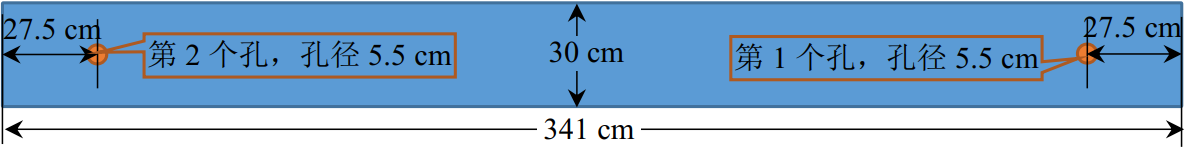
\includegraphics[width=0.7\textwidth]{pic/dragon-head.png}
\caption{龙头的俯视图}
\label{fig-dragonhead}
\vspace{1.0cm}

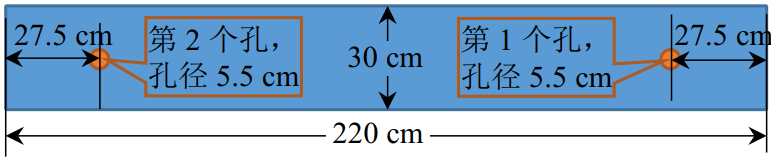
\includegraphics[width=0.7\textwidth]{pic/dragon-body.png}
\caption{龙身和龙尾的俯视图}
\label{fig-dragonbody}
\vspace{1.0cm}

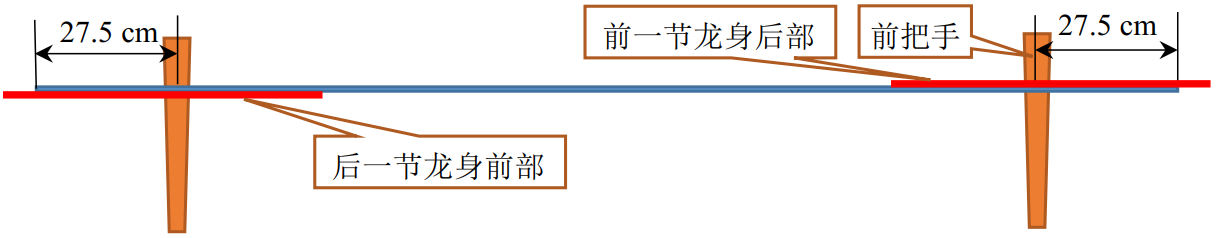
\includegraphics[width=0.7\textwidth]{pic/ban deng.png}
\caption{板凳的正视图}
\label{fig-bandeng}
\end{figure}

为此我们需要解决以下五个问题：
\begin{enumerate}
    \item 舞龙队沿螺距为 55 cm 的等距螺线顺时针盘入， 各把手中心均位于螺线上。 龙头前把手的行进速度始终保持 1 m/s。 初始时， 龙头位于螺线第 16 圈 A 点处（ 见图 4）。 请给出从初始时刻到 300 s 为止， 每秒整个舞龙队的位置和速度，将结果保存到文件 result1.xlsx 中。同时在论文中给出 0 s、 60 s、 120 s、 180 s、 240 s、 300 s 时， 龙头前把手、 龙头后面第 1、51、 101、 151、 201 节龙身前把手和龙尾后把手的位置和速度。
    \item 舞龙队沿问题 1 设定的螺线盘入，请确定舞龙队盘入的终止时刻，使得板凳之间不发生碰撞（即舞龙队不能再继续盘入的时间）， 并给出此时舞龙队的位置和速度，将结果存放到文件 result2.xlsx 中。 同时在论文中给出此时龙头前把手、龙头后面第 1、 51、 101、 151、 201 条龙身前把手和龙尾后把手的位置和速度。
    \item 从盘入到盘出，舞龙队将由顺时针盘入调头切换为逆时针盘出， 这需要一定的调头空间。 若调头空间是以螺线中心为圆心、 直径为 9 m 的圆形区域（见图 5）， 请确定最小螺距，使得龙头前把手能够沿着相应的螺线盘入到调头空间的边界。
    \item 盘入螺线的螺距为 1.7 m， 盘出螺线与盘入螺线关于螺线中心呈中心对称， 舞龙队在问题 3 设定的调头空间内完成调头， 调头路径是由两段圆弧相切连接而成的 S 形曲线， 前一段圆弧的半径是后一段的 2 倍，它与盘入、盘出螺线均相切。 能否调整圆弧，仍保持各部分相切，使得调头曲线变短？龙头前把手的行进速度始终保持 1 m/s。 以调头开始时间为零时刻，给出从−100 s 开始到100 s 为止，每秒舞龙队的位置和速度，将结果存放到文件 result4.xlsx 中（模板文件见附件）。同时在论文中给出−100 s、 −50 s、 0 s、50 s、 100 s 时， 龙头前把手、龙头后面第 1、51、 101、 151、 201 节龙身前把手和龙尾后把手的位置和速度。
    \item 舞龙队沿问题 4 设定的路径行进， 龙头行进速度保持不变，请确定龙头的最大行进速度，使得舞龙队各把手的速度均不超过 2 m/s。
\end{enumerate}


%%%%%问题分析%%%%%
\section{问题分析}
\subsection{问题一分析}
针对问题一，本文首先将舞龙队盘入运动抽象为等距螺线上的参数化运动问题，通过已知螺距与初始位置建立螺线的极坐标表达形式，从而将每节板凳把手的空间位置统一表示为螺线参数$\theta$的函数。由于龙头前把手沿螺线以恒定速度 1 m/s 运动，其位置变化可转化为螺线弧长随时间线性变化的问题，因此本文通过“弧长—角度”关系实现对龙头$\theta(t)$的数值反解，从而逐时刻确定龙头在螺线上的位置。

在此基础上，考虑到各节板凳之间通过固定孔距刚性连接，整条舞龙队可视为沿螺线排列的离散约束链结构。因此，本文采用由前向后的递推方式：以龙头位置为起点，根据相邻两节之间的固定距离约束，逐节求解其对应的螺线参数$\theta$，从而依次确定所有板凳在每一时刻的位置分布。同时，在速度计算方面，通过对螺线参数随时间的变化关系进行传播，建立相邻两节之间角速度的递推关系，从而得到全队各节的速度大小。最终实现对整个舞龙队在 0–300 s 内逐秒位置与速度的数值求解。

\subsection{问题二分析}
针对问题二，本文在问题一建立的舞龙队运动模型基础上，进一步考虑板凳自身尺寸带来的空间碰撞约束。首先，根据问题一中计算得到的各把手中心位置，将每节板凳等效为具有实际长度和宽度的矩形刚体，从而建立板凳的几何表示模型。由于舞龙队沿螺线由外向内盘入，碰撞最可能发生于龙头进入已盘入区域的过程中，因此本文以龙头板凳为主要检测对象，根据龙头与后续板凳之间的螺线参数关系筛选可能发生碰撞的候选板凳，从而减少无效检测并提高计算效率。

在碰撞判定过程中，本文采用基于分离轴定理的矩形碰撞检测方法，计算龙头板凳与候选龙身板凳之间的最小间隙，并将该间隙作为判断舞龙队安全状态的依据。当最小间隙大于零时，认为舞龙队仍可继续盘入；当最小间隙小于等于零时，则认为板凳之间发生碰撞。在确定碰撞判据后，本文将终止时刻求解转化为时间搜索问题，通过逐层缩小时间步长确定碰撞发生的时间区间，并利用二分搜索进一步提高时间精度，最终获得舞龙队无法继续盘入的临界安全时刻，并输出该时刻各节板凳的位置与速度信息。

\subsection{问题三分析}针对问题三，本文将最小螺距求解转化为螺距参数下的可行性判断问题。考虑到调头空间由半径约束确定，本文以龙头当前半径作为盘入状态变量，建立给定螺距与龙头位置下的舞龙队空间构型模型，并利用问题一中的板凳连接约束递推求解各节板凳位置。

在碰撞约束处理方面，本文沿用问题二中的几何碰撞模型，将板凳等效为矩形刚体，并基于舞龙盘入过程中的碰撞特点，检测龙头与附近内层板凳之间的潜在碰撞关系。采用分离轴定理（SAT）计算板凳间最小净间隙，以判断当前螺距是否满足调头要求。对于给定螺距，本文通过多尺度半径搜索确定盘入全过程中的最小安全间隙；随后将螺距求解转化为单调可行性问题，利用二分搜索算法逐步逼近安全与不安全的临界螺距，最终获得满足调头空间约束的最小螺距。

\subsection{问题四分析}

\subsection{问题五分析}

%%%%%准备工作%%%%%
\section{初步准备}
\subsection{模型假设}
\begin{enumerate}
    \item 盘龙过程按照等距螺线盘入，对于未进入预设等距螺线的龙身龙尾部分，认为其也处于相同螺距的螺线上
    \item 假设板凳龙的板凳把手在运动中视为质点，板凳为矩形刚体，只考虑其形状，忽视实际厚度
    \item 假设板凳龙运动过程中只有把手位于螺线上，板凳的相对位置由前后把手与矩形形状决定
    \item 假设板凳间的连接视为铰链连接，连接点为把手，存在相对转动但忽视摩擦力
    
\end{enumerate}

%%表%%
\subsection{符号说明}
本文所使用的符号及说明如下表所示。
\begin{table}[htbp]
\centering
\zihao{5}

\caption{符号说明}
\begin{tabular}{ccc}
\toprule
符号 & 说明 & 单位 \\
\midrule
$\rho$ & 极径 & m \\
$\theta$ & 极角 & rad \\
$d$ & 螺距 & m \\
$v$ & 龙头前把手前进速度 & m/s \\
$d_1$ & 把手中心到最近板头距离 & m \\
$d_2$ & 半个板宽 & m \\
$M_i$ & 第i个板凳的前把手\\
$l_i$ & 第i块板凳前后把手中心所在直线 & \\
$l$ & 板凳前后把手中心距离 & m \\
$A_1$ & 龙头前外部角点 & \\
$A_2$ & 龙头后外部角点 & \\
$A_3$ & 第一节龙身前外部角点 & \\
$A_4$ & 第一节龙身后外部角点 & \\
$d_{ij}$ & 角点$A_j$与直线$l_i$的距离 & m \\
$O_1$ & 第一段圆弧圆心 & \\
$O_2$ & 第二段圆弧圆心 & \\
$\phi$ & 第一段圆弧所对圆心角 & rad \\
$D$ & 调头空间直径 & \\
\bottomrule
\end{tabular}

\vspace{0.5em}
\parbox{0.9\textwidth}{
\zihao{5}
注：其他符号已在相应部分中说明。
}
\end{table}
\FloatBarrier
%%%%%模型建立与求解%%%%%
\section{模型建立与求解}
\subsection{问题一的模型建立与求解}
\subsubsection{模型建立}

将等距螺线表示为
\begin{equation}
    r=b\theta
\end{equation}
从而将二维位置$(x,y)$转换为单参数$\theta$表示。

龙头沿等距螺线以恒定速度1m/s运动，故其位置变化等价为螺线弧长的线性减少：
\begin{equation}
    s(t)=s_0-vt
\end{equation}
进而可通过数值来反解得到每一时刻$\theta_0(t)$。

在龙身递推方面，由于各板凳通过固定孔距连接，第i节满足距离约束：
\begin{equation}
    ||P_i-P_{i-1}||=d_i
\end{equation}
因此可由龙头开始，向龙尾方向逐节递推$\theta_i(t)$，形成链式递推结构

至于速度，使用求导方法，对螺线位置函数求时间导数，得到$\theta'$，再由链式关系传播至各节，最终计算速度大小。

在具体的数值求解上，由于$\theta$与距离约束均为非线性方程，故采用逐时间步+逐节点的数值递推求解。

\subsubsection{计算结果}

\subsection{问题二的模型建立与求解}
\subsubsection{模型建立}
在盘入过程中，龙头以恒定速度不断往内盘入，这让螺旋曲线的曲率越来越大，而板凳长度不可变，这使得相邻的两个板凳之间的夹角越来越小，于是越来越容易发生碰撞。

首先，为了简化后续计算过程，先用反证法证明一下第一次碰撞必然是龙头与内两层板凳发生的碰撞。我们假设一个龙头之外的板凳在t时刻时发生了第一次碰撞，那在t时刻之前必有一个时刻龙头已经到达过这个位置，那么龙头也发生了碰撞，所以原假设不成立，所以必然是龙头发生第一次碰撞。

在碰撞检测中，仅根据把手中心点之间的距离并不能准确反映板凳之间是否发生碰撞，因为板凳具有一定的长度和宽度。

在盘入过程中，通过两个把手$M_1$和$M_2$位置，可以通过如下公式确定板凳所在的矩形四个顶点位置

(在此处插入图片及公式)TODO

这样就可以把板凳碰撞转化为求解两个矩形相交的问题，为了解决矩形相交问题，接下来引入分离轴定理。

分离轴定理即对于两个凸多边形，若存在某一方向，使得二者在该方向上的投影区间互不重叠，则两个图形一定不相交；若在所有候选分离轴上的投影区间均发生重叠，则两个图形相交。该判别方法称为分离轴定理。由于矩形的候选分离轴只需取两矩形各自的长边方向和宽边方向，因此计算量较小，适合用于本题中大量板凳之间的碰撞检测。



\subsubsection{计算结果}

\subsection{问题三的模型建立与求解}
\subsubsection{模型建立}
\subsubsection{计算结果}

\subsection{问题四的模型建立与求解}
\subsubsection{模型建立}
\subsubsection{计算结果}

\subsection{问题五的模型建立与求解}
\subsubsection{模型建立}
\subsubsection{计算结果}

%%%%%评价%%%%%
\section{模型评价}
\subsection{模型的优点}

\subsection{模型的缺点}

%%%%%总结%%%%%
\section{总结}

本文通过对“板凳龙”问题的分析与建模、编写代码与计算结果，发现了...

%%%%%参考文献%%%%%s
\begin{thebibliography}{99}   % 99 是最大编号宽度
\bibitem{ref1} 张三, 李四. 论文标题[J]. 计算机学报, 2023, 46(1): 1-10.
\bibitem{ref2} Knuth D E. The TEXbook[M]. Addison-Wesley, 1984.
\end{thebibliography}

\section*{附录}
\appendix
\subsection*{文件清单}       % 显示为“附录 A 算法证明”
\subsection*{代码}       % 显示为“附录 B 数据表格”

\end{document}
